\chapter{SDN中LDoS方案设计}
\label{cha:design}
本章的主要内容为LDoS防御方案的设计。首先,对LDoS的特征进行分析,找到防御LDoS的关键点点。然后,根据防御LDoS的要点,结合SDN的优势设计了SDN中防御LDoS的两种方案。最后,对两种方案的设计思想和实现方案进行探索和分析。本文是基于SDN中最经典的OpenFlow协议完成设计的。

\section{SDN中LDoS防御的关键点分析}
\label{chap4:keyanalysis}
前文已经对LDoS攻击的攻击形式有了说明,本文首先分析单一攻击源的LDoS攻击实现的关键点并找到合适的防御机制。LDoS攻击的核心思想就是通过周期性的引发TCP流丢包,触发TCP拥塞控制机制或者超时重传机制降低TCP流的吞吐量,最后达到以极低的流量使TCP流异常的目标。因此,本文防御LDoS有两种核心思想,第一种是采取措施使TCP流不丢包,第二种是找到并限制攻击源。

第一种思想是采取措施使得TCP流不丢包。通过前文可知,TCP流的丢包是由于LDoS的速率太高拥塞队列导致的。所以,只要交换机保护TCP流的最低通信需求,则TCP不会因为收不到任何包而进入超时重传状态。在SDN网络中,带宽保障可以通过SDN中特有的meter规则去实现,使用meter规则限制其他流的最高速率从而给TCP流提供有最低速率保障,则LDoS无法通过拥塞队列强迫TCP流完全丢包。从而达到防御LDoS攻击的效果。但是,这样的做法在LDoS攻击的突发到达的时候,速率依然会降得很低,而拥塞窗口也会相应的减小,因此,这种思想只能减轻攻击所造成的危害,但是不能完全消除LDoS攻击对TCP流的影响。

第二种思想是找到并且限制攻击源。在SDN网络中,所有的数据转发都是由流表规则匹配完成的,因此,在SDN中可以实现流级别的数据分析。由于LDoS攻击拥塞了某个交换机的队列才能实现攻击,因此,可以在交换机的端口处检测LDoS是否存在。LDoS攻击作为一个周期性的“方波”是能够由周期性来确认的,因此,在端口处只要能够确认有周期性的吞吐量变化,就能够确认攻击,再之后通过流级别的分析判断攻击流,最后,再对判断出来的攻击流的攻击源进行限制。使用这种思想来防御LDoS攻击就能够完全消除LDoS攻击流对TCP流的影响,但是,在攻击开始的时候TCP流会受到一定的影响,可能会出现部分TCP流进入超时重传状态,影响吞吐量。

\section{SDN中基于带宽保障的LDoS防御方案}
\label{chap4:bandguatee}

保证TCP流不进入超时重传状态,防御方案必须保证TCP流无论在什么情况下都不能丢包,结合SDN的特性,该方案结合OpenFlow的Meter规则来实现,可以最大程度利用SDN网络可以自由制定网络规则的特性。

首先,分析Meter规则是如何在SDN中运行的,才能制定Meter规则防御LDoS攻击。Meter规则允许SDN实现各种各样的服务质量(Quality of Service,QoS)配置,其中就包括了速率限制。Meter规则能够直接与SDN中的流表规则绑定,这个Meter规则可以测量和控制所有与之绑定的流表规则的聚合速率,因此,Meter规则可以用来限制除TCP流以外的所有流聚合的速率。

\begin{table}[htbp]
	\centering  % 显示位置为中间
	\caption{Meter规则}  % 表格标题mn9GFFFFFFFFFFFFFFFFFFFFFFFFFFFFFFFFFFFFFFFFFFFFFFFFFFFFFFFFFFFF
	\label{table:meter}  % 用于索引表格的标签
	%字母的个数对应列数,|代表分割线
	% l代表左对齐,c代表居中,r代表右对齐
	\begin{tabular}{|c|c|c|}  
		\hline  % 表格的横线
        Meter Identifier & Meter Bands& Counters \\  % 表格中的内容,用&分开,\\表示下一行
        \hline
		
	\end{tabular}
\end{table}

表\ref{table:meter}为SDN的Meter规则的主要内容。Meter Identifier是一个32比特的无符号整数,它能够用于唯一标识一个Meter规则。counters是统计与meter绑定的流表规则的统计相关数据,随时更新。其中,最重要的是Meter Bands,它是Meter规则控制和限制绑定聚合流的速率和处理包方式的的部分。需要注意的是,每个Meter规则可以匹配多个Meter Band。表\ref{table:meterbands}为一个Meter Band部分,它由五个部分组成,首先是Band Type部分,这直接定义了速率超过限定速率以后,后面的包是如何处理的。此处有两种选项:一种为\emph{drop},这样它该Meter规则就可以被用来限制速率;一种为\emph{dscp remark},这样就能增加数据包IP头中DSCP字段的丢弃优先级,可用于定义不同级别的服务。第二个参数是Meter规则限制的速率,它定义Meter规则最低适用的速率,若是速率高于该参数的数据包则需要根据Meter规则进行处理。Counters表示被该Meter Band处理的包的统计数据。Burst参数是本文需要调的一个重要参数,该参数定义了Meter Band的粒度。Type specific arguments表示band types有特殊的参数。

\begin{table}[htbp]
	\centering  % 显示位置为中间
	\caption{Meter Band}  % 表格标题
	\label{table:meterbands}  % 用于索引表格的标签
	%字母的个数对应列数,|代表分割线
	% l代表左对齐,c代表居中,r代表右对齐
	\begin{tabular}{|c|c|c|c|c|}  
		\hline  % 表格的横线
        Band Type & Rate & Burst & Counters & Type specific arguments \\  % 表格中的内容,用&分开,\\表示下一行
        \hline
		
	\end{tabular}
\end{table}

此方案使用Meter规则来实现对非TCP流的速率限制,这样就能够对LDoS攻击进行限制。但是,由于LDoS攻击具有一定的特殊性,普通配置Meter规则无法限制LDoS攻击,需要特殊的配置。首先,由于LDoS攻击会拥塞某个端口的队列,所以,对于每个激活的端口,都应当配置一个相应的Meter规则进行限制,对于从端口处发送非TCP数据的流表规则需要与该端口的Meter规则进行绑定,受该Meter规则的束缚。接下来,Meter规则的粒度也需要特殊的配置,默认的状态下,Meter规则是以1秒作为统计单位进行速率限制的,由于LDoS攻击的平均速率并不能满足Meter规则限制的需求,因此Meter Band设置的Burst参数需要重新配置。接下来,需要设置Rate参数的大小来限制非TCP聚合流的速率,设置的参数数值大了会影响其他正常流的速率,设置的值过小会使TCP流的窗口降至极小的程度,达不到限制LDoS攻击的效果。因此,该参数对窗口大小的影响非常重要。


基于带宽保障的LDoS防御方案可以分为两个模块完成。流程图如\ref{fig:meter-solution}所示。防御方案的第一模块为预配置Meter规则模块,控制器首先会检测所有激活端口,并给每个端口分配一个Meter规则,Meter规则需要调节Burst参数使得粒度在RTT级别大小,这样才能够有效的限制LDoS攻击的速率。其次,设置合理的Rate参数保证TCP流不进入超时重传机制的同时使滑动窗口不至于变得太小。设置Band Type为drop,这样就丢弃所有超速的包,可以保障了TCP流有一定的带宽可以使用。防御方案的第二个模块为流处理模块,有一个流进入交换机,则需要对该流进行区分处理。若是该流为TCP流,则该TCP流的流表不需要绑定任何Meter规则,这样它就不会被Meter规则所束缚,可以按照TCP拥塞控制的机制进行速率的控制。若是该流不是TCP流,则需要绑定Meter规则以保证该流不会对TCP流造成损害,特别是当该流为LDoS攻击流的时候,由于速率被控制,队列不会被该流所拥塞而造成TCP流丢包,TCP流就不会进入超时重传状态。


%图 窗口与burst size的关系图,窗口与限制速率关系	有无防御机制吞吐量对比图

\begin{figure}
    \centering
    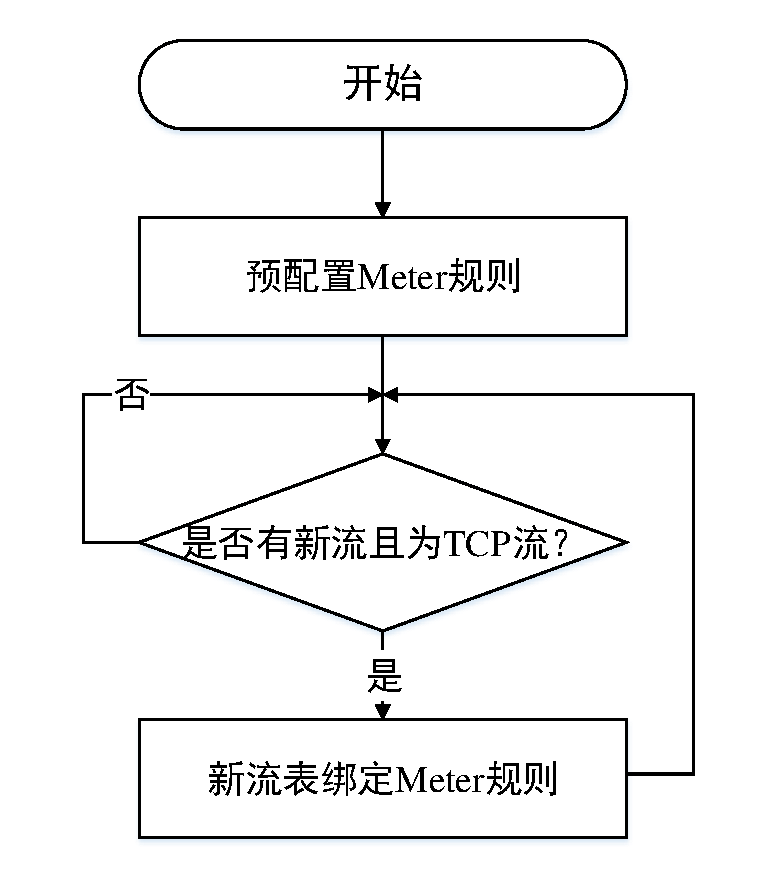
\includegraphics[scale=1]{meter-solution}
    \caption{基于带宽保障的LDoS防御方案流程图}
    \label{fig:meter-solution}
\end{figure}


\section{SDN中基于动态周期性检测的LDoS防御方案}
\label{chap4:SoftGuard}
已有SDN防御方案无法对LDoS限制的时候,为了保证SDN网络的正常传输,本文提出了基于动态周期性检测的方案。作为一个基于SDN的轻量级防御方案,该方案能够准确地识别并且有效的限制LDoS攻击。该方案分为三个模块,异常检测模块、攻击定位模块和攻击限制模块。每个模块都有特定的攻击,只有在一定的条件下激活才能发挥作用。因此,也最大程度的减轻了系统的负担。该方案是基于SDN中流表规则实现的,通过流表规则,SDN控制器能够获取交换机中各种有用的信息。

\subsection{SDN中相关流表规则分析}
\label{chap4:flowruleanalysis}

流表规则是SDN交换机中很重要的部分,所有的经过交换机的数据包都需要经过流表规则进行处理,这些数据包会优先寻找优先级比较高的流表规则进行匹配,这些流表规则可能有很多指令规则,其中比较重要的有两种,一种是将包从端口转发出交换机,另一种是转给交换机内的其他流表规则处理。表\ref{table:flowrule}为流表规则的主要内容。根据需求合理的配置流表规则的参数,能够实现对LDoS攻击的检测与限制。

本文对流表规则重要的部分进行分析,制定适合特制的流表来实现LDoS攻击的防御。在流表规则中,最重要的三个部分是匹配域(Match Fields)、优先级(Priority)和指令(Instructions)。匹配域是一般是由入端口和数据包头部组成的,也有其他可选项区域。优先级(Priority)是用来区分数据包优先匹配的规则的,若是同一个数据包同时匹配两个流表规则的匹配域,则该数据包会优先按照优先级高的流表规则的指令操作。在通过匹配域和优先级可以使数据包确定匹配的流表规则,若是没有匹配上流表规则,就会将该数据包的包头上传控制器,请求相应的流表规则。在确认了流表规则之后,该数据包会按照流表规则的指令完成操作。流表规则还具备数据统计的功能,其中的计数器(Counters)就记录了很多重要的信息,其中包括了转发的数据包的数量和字节数,每当匹配到数据包时,计数器中的数据就会实时更新。流表规则中的Timeouts参数包括两个timeout参数,idle\_timeout和hard\_timeout,idle\_timeout若是一个非0的数值,则流表规则在匹配最后一个包之后的idle\_timeout给定的时间后移除,idle\_timeout为0,则该参数不影响流表规则。hard\_timeout是若为非0的数值,则流表规则不管有没有匹配数据包,都会在hard\_timeout给定的时间后移除。hard\_timeout为0,则该参数不影响流表规则。若是idle\_timeout和hard\_timeout都为0,则流表规则永远存在,而且除了特定的指令外不会被删除。Cookie部分是控制器用于标识流表的不透明数据,该数据可以用来获取特定流表规则的信息,在处理数据包的时候不适用。Flags字段可用于出发特殊的消息给控制器。


\begin{table}[htbp]
	\centering  % 显示位置为中间13
	\caption{流表规则}  % 表格标题
	\label{table:flowrule}  % 用于索引表格的标签
	%字母的个数对应列数,|代表分割线
	% l代表左对齐,c代表居中,r代表右对齐
	\begin{tabular}{|c|c|c|c|c|c|c|}  
		\hline  % 表格的横线
        Match Fields & Priority & Counters & Instructions & Timeouts & Cookie & Flags \\  % 表格中的内容,用&分开,\\表示下一行
        \hline
		
	\end{tabular}
\end{table}

控制器通过以恒定的速率进行周期性的查询可以获得每个流表规则中计数器的速率。对于不同应用,通过选择合适采样的周期可以尽可能减少控制器的带宽负载的同时也可以尽可能提高服务的质量。本文将每次查询的间隔时间长度标记为$T_s$,将以此采样间隔内的平均速率当做采样时刻的速率,用于不同的服务。公式\ref{eqa:rate}展示了从流表规则的数据中获取流表规则速率的方式。

\begin{equation}
	\label{eqa:rate}
	S(t) = \frac{Counter\_bytes(t) - Counter\_bytes(t - T_s)}{T_s}
\end{equation}

\subsection{总体设计}
\label{chap4:overview}

基于动态周期性检测的LDoS防御方案有三个模块,异常检测模块、攻击定位模块和攻击限制模块。整体框架如图\ref{fig:architecture}所示。其中异常检测模块是在交换机中给每个端口都安装了特制的流表规则用于统计监测TCP的聚合流量。由于异常检测模块并没有对所有流表规则进行检测,这样就减少了对于控制器的带宽开销。当异常检测模块检测到某个端口聚合TCP吞吐量下降的时候,就会激发攻击定位模块来在这个异常端口处确认LDoS攻击、识别LDoS攻击流、并定位攻击源。确认LDoS攻击的关键点就是查看端口的聚合吞吐量是否存在周期性,由于LDoS攻击是由周期性的脉冲流组成的。攻击定位模块设计了适应性快速傅里叶变换(Fast Fourier Transform,FFT)方法来预测LDoS攻击的周期。除此之外,攻击定位模块还是用了平均欧氏距离(Mean Euclidean Distance,MED)从所有经过异常端口的流中识别出LDoS攻击流,然后通过SDN的全局视野找到攻击流的源端。最后,攻击限制模块将在LDoS攻击源的入口交换机处安装相应的限制规则以限制LDoS攻击流。

\begin{figure}
    \centering
    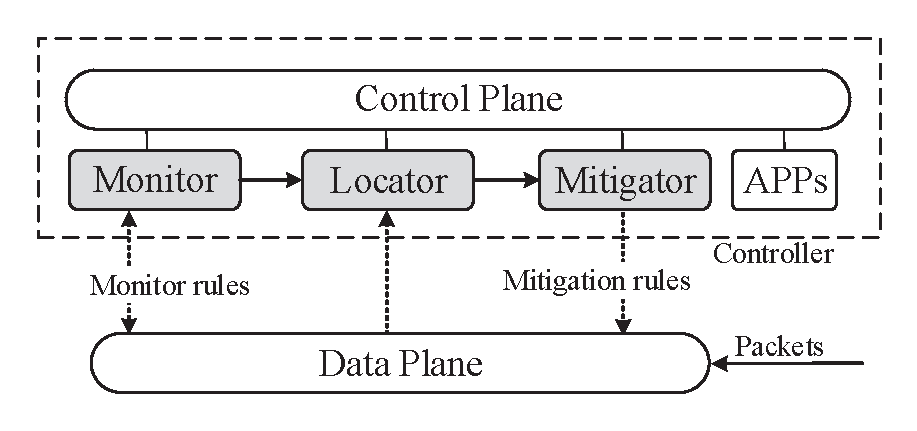
\includegraphics[scale=0.75]{architecture}
    \caption{基于带宽保障的LDoS防御方案流程图}
    \label{fig:architecture}
\end{figure}

\subsection{异常检测模块}
\label{chap4:Monitor}
异常检测模块的作用是在交换机上的每个端口处检测可能存在的LDoS攻击,并且激活其他模块来确认LDoS攻击。异常检测模块在每个交换机上安装检测流表规则在端口上来检测LDoS攻击。这些流表规则能够统计每个端口的聚合TCP吞吐量。异常检测模块通过周期性的获取这些流表规则的计数器数据就可以获知聚合TCP吞吐量变化情况。

异常检测模块首先从所有的数据包中分离出TCP数据包。然后,TCP数据包通过与这些特制的流表规则匹配,统计数据。接下来,再将这些TCP数据包转发给其他正常的流表规则进行处理。这些特制流表的匹配规则的匹配域加入转出端口信息,同时将优先级置为最高,以保证这些流表规则优先匹配数据包以统计TCP流的信息。接下来,特制的流表规则的指令为转发给其他正常流表规则进行处理,保证了这些流表规则只会统计TCP流的信息而不会干扰数据的传输。同时,异常检测模块需要把这些特制流表规则的idle\_timeout和hard\_timeout都设置为0以保证特制流表规则不会被删除,可以持续做数据的统计。

在交换机上安装特制流表规则后,异常检测模块按照算法\ref{alg:detection}检测聚合TCP吞吐量状态,若是聚合tcp吞吐量持续下降,则发现聚合TCP吞吐量下降明显则判断LDoS攻击可能出现,异常检测模块将会激活攻击定位模块来进行更深入精确的检测。算法\ref{alg:detection}展示了检测TCP吞吐量异常的伪代码。输入由吞吐量下降判定阈值$\alpha$和检测所得的序列$S$组成。输出为检测所得的结果$s$。$c$记录吞吐量持续下降的时间。如果$c$超过一个阈值$M$,$s$将会被标记为吞吐量异常,以此表示可能存在的LDoS攻击。同时检测到吞吐量异常的端口将被标记为异常端口。考虑控制器的带宽负载和模块的效率,设置异常检测模块的采样周期$T_s$为0.5秒,每次检测的时间长度为5秒。

\floatname{algorithm}{算法}
\renewcommand{\algorithmicrequire}{\textbf{输入:}}
\renewcommand{\algorithmicensure}{\textbf{输出:}}
\begin{algorithm}
	\small
	\caption{聚合TCP吞吐量异常检测}
	\label{alg:detection}
	\begin{algorithmic}[1]%ÿÐÐÏÔʾÐкÅ
	\Require $\alpha, S$;
	\Ensure $s$
	\State $c \gets 0$;
	\State $s \gets $吞吐量正常;
	\For{$(i=2 \rightarrow {len(S)})$}
		\If {$S_{i} < {\alpha} * S_{i - 1}$}
			\State $c \gets c + 1$;
		\Else 
			\State $c \gets 0$;
		\EndIf
		\If {$c {\ge} M$}
			\State $s \gets$ 吞吐量异常;
		\EndIf
	\EndFor
	\State \Return $s$
		
	\end{algorithmic}
\end{algorithm}

\subsection{攻击定位模块}
\label{chap4:Locator}

在异常检测模块激活了攻击检测模块之后,攻击检测模块对异常检测模块检测出的异常端口进行分析,确认LDoS攻击并识别LDoS攻击流。供给定位模块分为四个步骤。第一步,攻击定位模块对异常端口的总吞吐量进行二值化。第二步,攻击定位模块通过这些二值化后的吞吐量推断出异常端口吞吐量是否存在周期性。如果异常端口吞吐量存在周期性,则供给定位模块将确认异常端口正在被LDoS攻击所影响,因此,本文将确认被LDoS攻击所影响的端口称为受影响端口。攻击定位模块使用算法\ref{alg:port_locate}来确认异常端口是否为受影响端口。第三步,使用序列相似性来识别攻击流,通过平均欧式距离方法来判断攻击流。最后一步,找到攻击流的入口交换机上的端口,并且通知攻击限制模块来限制攻击流。




\subsubsection{吞吐量二值化}
\label{chap4:binarization}
通过采样获得的吞吐量序列在进行周期性判断之前需要进行处理。端口统计的数据包除了潜在的LDoS攻击数据包,也可能会包含在其他良性的流量影响周期性的判断。这些良性流量括三类:
\begin{itemize}
	\item 不会受到LDoS攻击和网络拥塞影响的UDP流
	\item LDoS未影响到的TCP流
	\item 其他经过该端口的更底层的数据流
\end{itemize}
这些良性流量不具备周期性,而且速率相较于LDoS的突发速率$R$要小很多。为了减少这些良性流量的影响,同时也为了更加便于提取周期性,攻击定位模块需要对流量进行二值化。攻击定位模块使用了阈值法进行二值化,假设该序列的最大吞吐量的值为$S_m$,设定阈值为$\beta$,则吞吐量序列值中高于$\beta S_m$的地方置为1,吞吐量序列值中低于$\beta S_m$的地方置为0,这样就可以得到二值化序列。

\subsubsection{流量周期性检测}
为了确认LDoS攻击,异常检测模块需要对吞吐量的二值化序列进行周期性的检测。假设某异常端口有周期为$T_r$的聚合流量,控制器通过对异常端口的数据以周期$T_s$进行采样。


\begin{algorithm}[H]
	\caption{动态搜索受影响的端口}
	\label{alg:port_locate}
	\begin{algorithmic}[1]
		\Require $~{\epsilon}, p$;
		\Ensure $s, T_s, T$;
		\State $T_s \gets T_i$;
		\State $T \gets \infty$; 
		\While{$T_s \ge T_e$}
		\State $seq \gets binarized\_sequence(T_s, p)$;
		\State $T_b \gets period\_mean\_fft(seq)$;
		\If {$abs(T - T_b * T_s)<\epsilon$}
		\State $s \gets$ 受影响;
		\State \Return $s, T_s, T$;
		\Else
		\State $T \gets T_b * T_s$;
		\State $T_s \gets T_s / 2$;
		\EndIf 
		\EndWhile
		\State $s \gets$ 不受影响;
		\State $T \gets 0$; 
		\State \Return $s, T_s, T$;
	\end{algorithmic}
\end{algorithm}